\section{Introduction}

\subsection{General Overview}

Evidence based decision making is increasingly presented as the best way to design public health policies at national and local levels \cite{abou-zahr_health_2005,shibuya_health_2005,bambas_nolen_strengthening_2005,mutemwa_hmis_2006,boerma_public_2013}.
The ability of statistics to offer rational basis to make decisions \cite{porter_trust_1996,desrosieres_politique_1993},
allied with progress in data collection and analysis techniques engender enthusiasm and hope in the ability of governments and other actors to design and implement analytical tools to improve the political and administrative processes, some even calling for a \textit{Data Revolution} in policy making \cite{independent_expert_group_on_a_data_revolution_for_sustainable_development_world_2014,center_for_global_development_delivering_2014}.

Meanwhile, if this principle seems to be set, what constitutes relevant evidence in an administrative context, and how it should be generated is less clear and depends on local contexts and traditions. Bergeron and Cassel note that knowledge and expertise of public health deciders are "a network involving many different actors, structures and tools, concepts and spatial and institutional arrangements" \cite{bergeron_savoirs_2014}. Producing knowledge for public health decision thus relies on localized and contextual approaches, that are not easily generalized to other situations. In the world of Global Health Metrics, the local and contextual dimension of statistical systems can sometimes be lost in an undue generalization. Meanwhile, the historical conditions of emergence of evidence generation systems for public health are very different in different parts of the world.

In most rich countries, a long history of public statistics development resulted in the emergence and stabilization of well defined data sources, of methods and of roles along which the generation of public statistics are produced. In these countries, there seems to be a convergence between the two values noted by Desrosières for statistics : statistics as a measure of reality, and statistics as a norm \cite{desrosieres_prouver_2014,desrosieres_administrator_1997}. Meanwhile, this should not hide the important historical debates and struggles that happened around simple objects such as averaging population statistics \cite{desrosieres_politique_1993,porter_trust_1996}, measuring hospital mortality or even collecting hospital data. As such, strong public health information systems really are the result of local equilibriums and of adaptations to local statistical cultures, but were started by individuals making ad-hoc use of different data sources and inventing and standardizing methods on the run\cite{lecuyer_medecins_1987}.

In sub-Saharan Africa, evidence generation for public health policy makers is in a very different situation. The weakness of statistical systems in sub-Saharan Africa has been well described and documented \cite{jerven_poor_2013}. Most sub-Saharan countries can't rely on a robust vital statistics system to plan population targeted intervention. National Health Information Systems are often considered weak \cite{abou-zahr_better_2010,kiberu_strengthening_2014}, and are affected by multiple uncoordinated demands for data collection and reporting. These demands may come from local authorities or from international donors and partners, which jeopardizes their accuracy \cite{sandefur_political_2013} . Moreover, the development of statistical systems in former colonies has been fostered in a context that had more to see with the need of control of colonial powers than with the search for evidence and decisional guidance \cite{appadurai_number_1996,cordell_couting_2010,gervais_how_2010}.

Colonial statisticians, often weakly skilled and trained \cite{cordell_couting_2010,kateb_gestion_1998}, nonetheless set the nomenclatures and conventions around which land and populations would be described and analyzed \cite{rambert_cartographie_1922,gervais_how_2010}. In the meantime, whereas European statistical systems were developed and structured by social activists willing to tailor welfare systems \cite{desrosieres_politique_1993,desrosieres_administrator_1997}, colonial statistical systems were geared towards efficient land administration and exploitation \cite{rambert_cartographie_1922,de_martonne_cartographie_1931} with little interest on population. In Sénégal in 1926, the first population estimation was made thanks to the availability of taxation records, but with no vital statistics records\cite{rousseau_population_1929}.

After the decolonizations, the administrative mindset of evidence generation was completed by the expert mindset of the developmental state \cite{bonneuil_development_2000}. Developmentalist expertise transformed African societies into objects of external studies and knowledge more than self-administering political entities, thus prolonging the outwards orientation of colonial statistics. The development and the rollout of neoliberal statistical management in the 90's, and the generalization of Monitoring and Evaluation (M\&E) for different projects \cite{desrosieres_prouver_2014} only strengthened and deepened this tendency. The low investment in data collection and excruciating exigency for unrealistic precision, the importation of external methods and definitions, the overarching generalization of categories for administrative simplicity, all these features can be traced back to colonial statistics.


\subsection{Work hypothesis}

My main work hypothesis is that the underwhelming performance of health information systems in developing countries stems from the top-down nature of their design and implementation.

By top-down I mean systems in which the purported usage of information calls for specific data collection and analytical tools. Most HMIS design recommendations for an ex-ante design of both data analysis and measure framework, from which data collection should be inferred. \cite{lippeveld_routine_2000,rhino_introducing_2003,daltilia_systeme_2005,health_metrics_network_framework_2008}. Also, M\&E guidelines such as those of Global Health agencies like the Global Fund exercise important drives on HMIS organization in sub-Saharan African countries on which they are imposing definitions, classifications and reporting methods, to provide sufficient information for the evaluation of funded programs\cite{the_global_fund_global_2014}.

The mindset behind these approaches is influenced both by the colonial administrative tradition, for which standardized statistical tools should provide a normed information, and by the developmentalist expertise tradition, along which an hyper directed data collection system is aimed at providing a unique and narrowly defined piece of knowledge. National Health Information Systems are then organized around these multiple narrowly defined needs for information, and are directed towards answering questions asked by level national or international specialists.

The critic of this type of statistical work is often conducted from a postmodernist perspective, questioning the structures and processes that produce statistical knowledge in developing countries. This critic, if it is sometimes useful to the practicing statistician, often poses a radical critic of the quantitative approach to public affairs, offering little place for incremental improvements \cite{rottenburg_world_2016}. In this dissertation, I explore ways through which this top-down approach to evidence generation in health systems can be reversed, to promote data analysis approaches that start with the data collected in the health systems, from which relevant information is extracted in an ad hoc way.

This approach is justified by two elements. First, the observation that strong national statistical systems emerged from both norm and local improvisation and trial and error \cite{lecuyer_medecins_1987,chaperon_information_1988}. Second, my approach is thought in the context of the development of the field of \textit{Data Science} as a complement or an adaptation of traditional statistics to new analytical tools and improved computational capabilities. I understand data science literally, meaning a scientific approach taking data as an object of study \textit{per se}, from which the analysis starts, and which conditions all subsequent reflection.

\subsection{Aims}

My principal aim will be to define, implement and test \textit{bottom up} approaches to improve Health Information Systems data use in developing countries. This aim will be reached through three specific aims, which address different key processes in health information systems. The Health Metrics Network defined the three main processes of Health Information Systems as the indicators definition and standardization, data sources and data management (database hosting, data cleaning and data processing) \cite{health_metrics_network_framework_2008}.

I will address each of these processes with a specific aim, and will explore how methods based on available data and processes can improve the performance of Health Information Systems.

\pgfdeclarelayer{background}
\pgfdeclarelayer{foreground}
\pgfsetlayers{background,main,foreground}
\begin{center}
 \begin {figure}[ht]
        \centering
\resizebox{\linewidth} {!} {
%\documentclass{standalone}
%\usepackage{tikz}

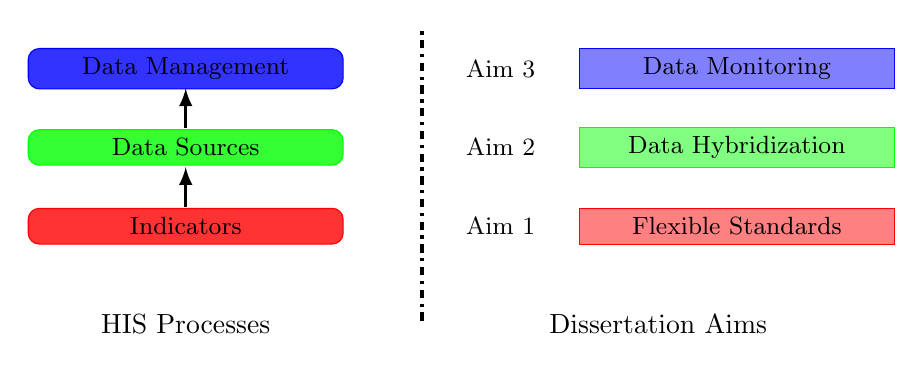
\begin{tikzpicture}

\node[draw , draw = blue ,  fill= blue!80 , minimum width=4cm , rounded corners] at (0,2){\small Data Management} ;
\node[draw , draw = green ,  fill= green!80 , minimum width=4cm , rounded corners] at (0,1) {\small Data Sources} ;
\node[draw , draw = red ,  fill= red!80 , minimum width=4cm , rounded corners] at (0,0) {\small Indicators} ;
\node[below] at (0,-1) {HIS Processes} ;

\draw[very thick , -latex] (0, 0.25) -- +(0,0.5) ;
\draw[very thick , -latex] (0, 1.25) -- +(0,0.5) ;
\draw[very thick , dash dot] (3, -1.2) -- +(0, 3.7) ;


\node[very thick] at (4,2){\small Aim 3} ;
\node[draw , draw = blue ,  fill= blue!50 , minimum width=4cm] at (7,2){\small Data Monitoring} ;
\node[very thick] at (4,1){\small Aim 2} ;
\node[draw , draw = green ,  fill= green!50  , minimum width=4cm] at (7,1){\small Data Hybridization} ;
\node[very thick] at (4,0){\small Aim 1} ;
\node[draw , draw = red ,  fill= red!50 , minimum width=4cm] at (7,0){\small Flexible Standards} ;
\node[below] at (6,-1) {Dissertation Aims} ;

\end{tikzpicture}

%\end{document}

}
\caption{HIS Processes and corresponding dissertation aims}
\label{fig:process_aim}
\end{figure}
\end{center}


\paragraph{Indicators / Flexible Standards} Defining categories and metrics based on which people are going to be counted is an essential piece of the statistical work \cite{desrosieres_politique_1993}. It is an essential step in the simplification involved in the activity of measurement. The field of Global Heath relies on important taxonomies, like the International Classification of Diseases and metrics, like the Disability Adjusted Life Years, to unify description and measurement of health across the globe, and allow comparison and benchmarking \cite{murray_towards_2007,murray_health_2008}. Meanwhile, at local level, the use of globally defined metrics may have its limits, as it does not allow adaptation to local contexts and situations. The measure of retention of HIV patients in care is an example of this. Understanding the outcome of patients after they enter care is essential to evaluating HIV care systems performance \cite{the_global_fund_global_2014}. Meanwhile, the high variation of results between programs and the low specificity of currently used indicators leads researcher to question the way Loss to Follow Up is defined and retention is measured globally \cite{chi_universal_2011,yehia_comparing_2012,grimsrud_impact_2013,forster_electronic_2008}. Using Electronic Medical Records, we will model how the measure of retention is affected by local contexts and data quality, and will explore better more robust ways to measure HIV care outcomes.

\paragraph{Data Sources / Data Hybridization} Unavailability of population data in a large number of countries is a well known issue \cite{mahapatra_civil_2007,mikkelsen_global_2015}. As a result, spatial distribution of populations, an essential piece of evidence to develop public health policies, is often unavailable at a policy relevant scale. To palliate these shortcomings, approaches for mapping of populations have been developed, involving the use of macro-level rasters of covariates such as land coverage or night light \cite{linard_population_2012,stevens_disaggregating_2015}. These approaches give interesting insights into how populations are distributed, and their output can easily be used for other public health work using the GPS coordinates system. Meanwhile, in situations with very low information on populations, the results of these top-down approaches is often little more than an overlay of covariates. Additionally, their results are hard to use for public health policy planning, as they do not link population to commonly used localization conventions such as places names. My third aim is to hybridize multiple data sources on population to produce a population map of Niger linked to the lowest level of population settlement possible.

\paragraph{Data management / Data Monitoring} Data quality is an important concern of Health Information Systems professionals \cite{shrestha_data_2000} who link it directly to the ability of Information systems to provide good information \cite{mphatswe_improving_2012}. The definition of data quality is directly linked to an idea of trustworthiness, which may affect the use of certain data sources to generate evidence \cite{gimbel_assessment_2011}, and the quality of health data receives a large amount of attention even from high level actors in Global Health \cite{abou-zahr_better_2010,lopez_better_2015}. The best way to ensure data quality is through routine audits of primary data \cite{ronveaux_immunization_2005}. Meanwhile, this approach is costly and may have some cost-efficiency issues. Additionally, it makes little use of historical data, which makes it vulnerable to issues in primary data. My second aim will be to develop a cost effective approach to data quality screening informed by historical data and including a notion of risk attached to data quality.

\subsection{Novelty and scientific contribution}

My dissertation is contributing to three main areas of research surrounding Health Information Systems. One is a research area mostly invested by the Information and Communication Technologies field (ICT) and interrogates the importance of local adaptation of information systems and its impact on the definition of standards. The second domain of relevance is more linked to the Global Health field, and on works that interrogate how data collected inside health systems can be used to best inform decision making. The last domain of contribution is mainly of interest for the statistical field, and explores the use of statistical methods in applied policy contexts.

\subsubsection{Local Adaptation and flexible standards}

In the ICT field, defining standards for data collection systems that can be implemented at local levels but respond to national or international norms. Jørn Braa, describing the approach that presides to the design and development of DHIS2 remarks that "the top-down and all-inclusive approach to standardization [is] common among ministries and central agencies" and pleads for a \textit{flexible standards} following the idea that "the individual standards must be crafted in a manner which allows the whole complex system of standards to be adaptive to the local context" \cite{braa_developing_2007}. The need for local adaptability of Information Systems is seen as a key issue of ICT in developing countries \cite{macfarlane_harmonizing_2005,walsham_research_2006,walsham_foreword:_2007,jacucci_standardization_2006} and thus some ICT solutions have been designed and explored in the forms of tools like the District Health Information Systems (DHIS2) or standards like the Open Health Information Exchange initiative (OpenHIE)

My two first aims explore ways in which indicators definition or data quality evaluation can be adapted to local situations. In both situations, flexibility is introduced through objective rules : specificity and robustness of the measure of retention in the first aim, and cost-effectiveness in the second aim. The two rules are different in nature, as one is internal, and based on the characteristics of the data while the other is external, and based on operational characteristics such as the cost of supervision. This approach is innovative, and can be applied to a diversity of questions. An extension of this work could also be the definition of methods for aggregation and comparison of locally defined metrics.

\subsubsection{Imperfect data Usage}


Health Information Systems data is often underused, or not used at all by its intended users\cite{health_metrics_network_framework_2008}. This underuse is often blamed on the  perceived bad quality of primary data that would make it unfit for statistical analysis
\cite{ronveaux_immunization_2005,makombe_assessing_2008,heunis_accuracy_2011,gimbel_assessment_2011,who_assessment_2011,hahn_where_2013,kihuba_assessing_2014,glele_ahanhanzo_data_2015}. Approaches to solve this issue have mainly focused on improving primary data quality to improve data use  \cite{braa_improving_2012,mutale_improving_2013,ledikwe_improving_2014,nisingizwe_toward_2014}, but some authors have also pointed to the possibility to use even imperfect routine data to answer specific public health questions\cite{gething_improving_2006,gething_information_2007,wagenaar_using_2016}. These approaches rely on the nature of routine data, which is usually highly dimensional and structured times series. This type of data enables the use of robust modeling methods at an adequate level of aggregation, to control and correct for data errors.

My dissertation contributes to this line of research in two different ways.

Aim 1 and 2 also offer improved insights in routine data quality and its impact on health indicators. Aim 1  explores a micro level modeling of data quality and its impact on the measure of patient retention. It will also define retention indicators less sensitive to data quality. Aim 2 is concerned with expected value imputation and aberrant values detection, which is an essential aspect of understanding data quality. It will also implement solutions  to analyze and display overdispersed data, often observed in health systems.

Aim 1 and aim 3 also examine methods to enrich the data used, using EMR metadata or  hybridizing different data sources. Both approaches are an extension of usual approaches to health data, and make full use of the richness of modern data collection tools, and of the wide availability of public data sources.

\subsubsection{Statistical methods for health data monitoring}

For our aim 2, I am interested in two types of literature that address issues of health data monitoring :
epidemiological surveillance and service quality monitoring. Epidemiological surveillance is interested in spotting changes of regime in reported counts of cases for different diseases, while quality control data, more inspired by an industrial approach to data monitoring, is interested in spotting outlying performances of specific units in a health system. In both literatures, a common algorithm for data inspection can be described in the three following steps :
\begin{enumerate}
    \item Impute expected domain of a variable under a null hypothesis
    \item Test the null hypothesis
    \item Display result for human decision
\end{enumerate}

How each of these steps is in effect implemented will be influenced by the specific approaches and expected information. The current reference approach to syndromic surveillance systems is the Farrington method \cite{farrington_statistical_1996}, modified by Noufaily to improve handling of seasonality and power of detection tests \cite{noufaily_improved_2013,salmon_advances_2016}. In this approach, a quasi-Poisson distribution of indicators is fit and the detection threshold is defined as a corrected Z-score for these expected distributions. In the quality monitoring literature, of Spiegelhalter \cite{spiegelhalter_statistical_2012} offers a good overview of methods in use, relying on Z-scores of observed distributions. The same approach is also described in a generic hierarchical modeling framework to identify outstanding facility level effects\cite{ohlssen_hierarchical_2007,jones_improved_2012}.

I will explore a combination of both approaches to provide actionable information on available data in a health system. Indeed, we will handle data quality screening as a surveillance issue, aiming at spotting aberrant data in time series, and will then implement quality monitoring algorithms to identify outlying facilities. Describing the result of the combination of these two approaches to analyze data distribution in space and time will be an innovative application of existing methods.

In the meantime, my implementation of  quality monitoring algorithms will differ from existing literature in an essential way. In most quality monitoring applications, the quantity of interest is the success of some type of procedure, measured by an outcome, of which death is usually the least desirable. In the context of Results Based Funding, on the other hand, the measure of success is much more a measure of access to a wide range of services. The denominator of such a measure is much less clear, as it is not defined at facility level, and there is often little information on target populations. I will thus need to define the null hypothesis in a multivariate or compositional way, stating that the relative importance of different indicators should be similar, modulo a stratification of health facilities. An approach to Z-Score combination is described by Spiegelhalter \cite{spiegelhalter_statistical_2012}, on which we will build to define a facility level measure of performance.


\subsection{Timeline}

Aim specific timelines are explained in more detail in sections \ref{timeline:aim1}, \ref{timeline:aim2} and \ref{timeline:aim3}. I will prioritize getting early results on Aim 2 to allow feedback and field testing from Bluesquare and have an opportunity to reorient my methods if needed. This will also leave time me to obtain potential additional data for Aims 1 and 3. All the aims should be finalized and papers written by the end of the first quarter of 2018, which would allow for a finalization of the dissertation by June 2018.


\begin{figure}[!ht]
	\begin{ganttchart}[vgrid ,
                    hgrid,
                    y unit chart=.6cm]{1}{18}
		\gantttitle{2017}{12}
		\gantttitle{2018}{6} \\
		\gantttitlelist{1,...,12}{1} \gantttitlelist{1,...,6}{1}\\

        \ganttset{bar/.append style={draw=red!40 , fill=red!40},
                    group/.append style={draw=red, fill=red}}
		\ganttgroup{Aim 1}{1}{16} \\
		\ganttbar{Data Extraction}{1}{4} \\
		\ganttbar{Modeling and Model estimation}{5}{6} \\
		\ganttbar{Cohort Simulation}{7}{9} \\
		\ganttmilestone{Sharing Cohort simulation results}{9} \\
		\ganttbar{Data Quality Impact}{10}{10} \\
		\ganttbar{Data Maturity}{11}{12} \\
		\ganttbar{Robust Measures of retention}{13}{14} \\
		\ganttmilestone{Sharing Final Results}{14} \\
		\ganttbar{Paper Writing}{15}{16} \\
		\ganttmilestone{Paper Submission}{16}\\

        \ganttset{bar/.append style={draw=green!40 , fill=green!40},
                    group/.append style={draw=green, fill=green}}
        \ganttgroup{Aim 2}{1}{16} \\
		\ganttbar{Data Extraction}{1}{3} \\
		\ganttbar{Name Matching}{1}{6} \\
		\ganttbar{Locality Mapping}{7}{9} \\
		\ganttmilestone{First complete map}{9} \\
		\ganttbar{Population Estimation}{10}{14} \\
		\ganttmilestone{Sharing Final Results}{14} \\
		\ganttbar{Paper Writing}{15}{16} \\
		\ganttbar{Dashboard Design}{15}{16} \\
		\ganttmilestone{Paper Submission}{16}\\

        \ganttset{bar/.append style={draw=blue!40 , fill=blue!40},
                    group/.append style={draw=blue, fill=blue}}
        \ganttgroup{Aim 3}{1}{11} \\
        \ganttbar{Data Extraction}{1}{1} \\
		\ganttbar{Data Quality Modelling}{2}{5} \\
		\ganttmilestone{Sharing Data Quality Models}{5} \\
		\ganttbar{Service Quality Monitoring}{6}{7} \\
		\ganttmilestone{Sharing Service Quality results}{7} \\
		\ganttbar{Operational Fine tuning}{8}{9} \\
		\ganttmilestone{Sharing Final Results}{9} \\
		\ganttbar{Paper Writing}{10}{11} \\
		\ganttmilestone{Paper Submission}{11}\\
	\end{ganttchart}
	\caption{Dissertation Timeline}
\end{figure}
